As can be seen in the section above, the model performs fairly well on all metrics: see Table~\ref{tab:resClasses}. The \gls{iou} is good, meaning that once an object is detected, the bounding box around that object is accurate. Class Accuracy is adequate, with the best performance being with the Celtic Fields, which are very characteristic and easily recognizable. Performance could be improved for the "Barrows" class, since it has the lowest accuracy of all the classes, and the most confused class. 


\begin{figure}[H]
  \centering
  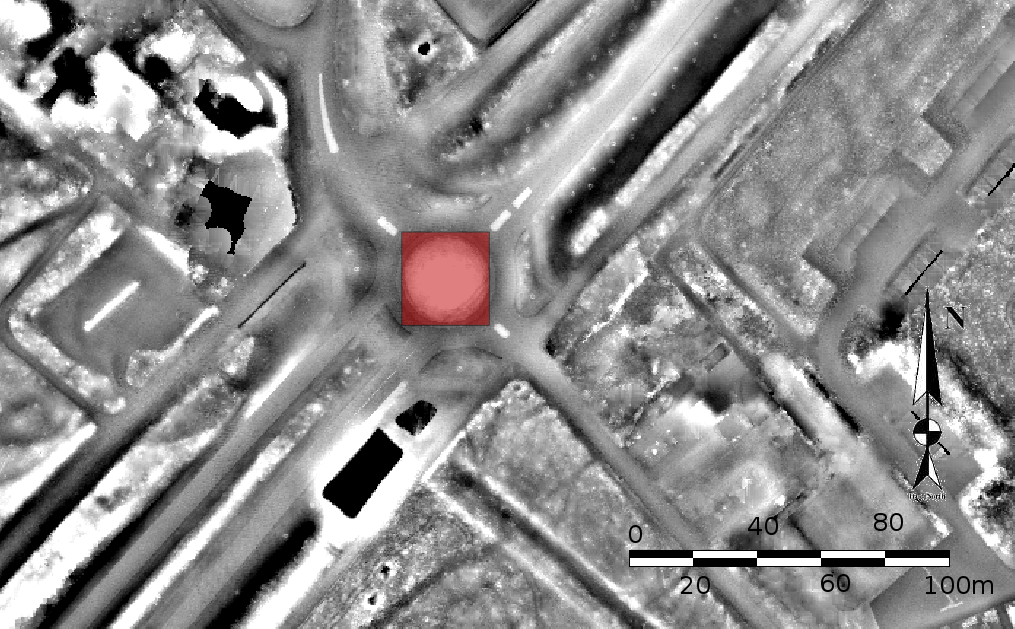
\includegraphics[width=0.8\textwidth]{wrongBarrow}
	\caption[]{Confusion between a roundabounts and a barrow. Details from a survey done in the region of the Veluwe, Central Netherlands.}
  \label{}
\end{figure}

Some errors do still occurs, especially with \textbf{roundabouts being confused for barrows, an issue already noticed in Verschoof-van Der Waart and Lambers\cite{wouter2019}}. While this might be an problem with the training of the network, it might also indicate that the \gls{lidar} survey do not hold enough informations to discriminate between those two type of objects, as discussed in Section~\ref{diffLidarNat}. 

This ties again with the fact that we are not training a model that is detecting archaeological objects, but simply objects. The model is incapable of infering the archaeological origin of the object based purely on appearance, as is exemplified with the roundabounts being mischaracterised as barrows. Creating a model capable of such a feat is much harder than simply training an object detector. Some kind of reasoning needs to be done to understand the archaeological properties of objects, or at least extracting more general and global information than can be done using local convolutions. This could be done using domain knowledge to post process the detection results and eliminate false positive. This has been done in a recent article by Verschoof-van der Vaart\cite{lamberVerschoof}, with location based ranking of barrows being used, with good success.   
